%This is a very basic  BE PROJECT PRELIMINARY template.

%############################################# 
%#########Author :  PROJECT###########
%#########COMPUTER ENGINEERING############


\documentclass[oneside,a4paper,12pt]{book}
\usepackage{graphicx}
\usepackage{titlesec}
\graphicspath{{diagrams/}}
\usepackage{enumerate}
\usepackage{geometry}

\geometry{a4paper,
  margin=30mm
}


\newcommand\tab[1][1cm]{\hspace*{#1}}
%\usepackage{showframe}
%\hoffset = 8.9436619718309859154929577464789pt
%\voffset = 13.028169014084507042253521126761pt

%\fancypagestyle{plain}{
%  \fancyhf{}
 % \fancyfoot[CE]{College_Name, Department of Computer Engineering 2015-16}
 % \fancyfoot[RE]{\thepage}
%}
%\pagestyle{fancy}
%\fancyhead{}
%\renewcommand{\headrulewidth}{0pt}
%\footskip = 0.625in
%\cfoot{}
%\rfoot{}

\usepackage[]{hyperref}
\usepackage{tikz}
\usetikzlibrary{arrows,shapes,snakes,automata,backgrounds,petri}

\usepackage{tabularx}

\usepackage[nottoc,notlot,notlof,numbib]{tocbibind}
\usepackage[titletoc]{appendix}
\usepackage{titletoc}
\renewcommand{\appendixname}{Annexure}
\renewcommand{\bibname}{References}

\setcounter{secnumdepth}{5}

\usepackage{float}
\usepackage{subcaption}
\usepackage{multirow}

\usepackage[ruled,vlined]{algorithm2e}

\begin{document}

\setlength{\parindent}{0mm}
\begin{center}
{\bfseries SAVITRIBAI PHULE PUNE UNIVERSITY \\}
 \vspace*{1\baselineskip}
{\bfseries A  PROJECT REPORT ON \\}
 \vspace*{2\baselineskip}
{\bfseries \fontsize{16}{16} \selectfont  `APPLICATION FOR MANAGING A 
\\ VETERINARY POLYCLINIC' \\
\vspace*{4\baselineskip}} 
{\fontsize{12}{12} \selectfont SUBMITTED TOWARDS THE
 \\PARTIAL FULFILLMENT OF THE REQUIREMENTS OF \\

\vspace*{2\baselineskip}}
{\bfseries \fontsize{14}{12} \selectfont BACHELOR OF ENGINEERING (Computer
Engineering) \\
\vspace*{1\baselineskip}} 
{\bfseries \fontsize{14}{12} \selectfont BY \\ 
\vspace*{2\baselineskip}} 
Shalini Prasanna  \hspace{24 mm} Exam No:B120204364  \\
T. Pavithra \hspace{34 mm} Exam No:B120204409  \\
Supriya Waghmare \hspace{23 mm} Exam No: B120204404  \\
Ashlesha Waikos \hspace{25 mm} Exam No:B120204424\\
\vspace*{2\baselineskip}
{\bfseries \fontsize{14}{12} \selectfont Under The Guidance of \\  
\vspace*{2\baselineskip}} 
Prof. Pranjali Deshpande\\
\vspace*{3\baselineskip}
\includegraphics[width=100pt]{collegelogo.png} \\
\vspace*{3\baselineskip}
{\bfseries \fontsize{14}{12} \selectfont DEPARTMENT OF COMPUTER ENGINEERING \\ 
\vspace*{2\baselineskip}
MKSSS'S CUMMINS COLLEGE OF ENGINEERING FOR WOMEN \\
PUNE
}
\end{center}

\newpage

{\bfseries \fontsize{16}{12} \selectfont \centerline{CERTIFICATE} 
\vspace*{4\baselineskip}} 

\centerline{This is to certify that the Project Entitled}
\vspace*{.5\baselineskip} 


{\bfseries \fontsize{14}{12} \selectfont \centerline{ `APPLICATION FOR MANAGING A VETERINARY POLYCLINIC'}
\vspace*{0.5\baselineskip}}

\centerline{Submitted by}
\vspace*{2\baselineskip} 
\centerline{Shalini Prasanna  \hspace{24 mm} Exam No:B120204364 } 
\centerline{T. Pavithra \hspace{34 mm} Exam No:B120204409  } 
\centerline{Supriya Waghmare \hspace{23 mm} Exam No:B120204404 }
\centerline{Ashlesha Waikos \hspace{25 mm} Exam No:B120204424 }
\vspace*{2\baselineskip}
is a bonafide work carried out by Students under the supervision of Prof. Pranjali Deshpande and it
is submitted towards the fulfilment of the requirement of Bachelor of Engineering (Computer Engineering).\\ \\ \\ \\ \\ \\ \\ \\ \\
\bgroup
\def\arraystretch{0.7}
\begin{tabular}{c c }

Prof. Pranjali Deshpande &  \hspace{50 mm} Dr. Supriya Kelkar \\								
Internal Guide   &  \hspace{50 mm} H.O.D \\
Dept. of Computer Engg.  &	\hspace{50 mm}Dept. of Computer Engg.  \\
\end{tabular}
%}
\begin{center}
\vspace*{4\baselineskip}
%\fontsize{12}{18}\selectfont 
{
Dr. Madhuri Khambete\\
Director\\
MKSSS'S Cummins College of engineering for Women  
}
\end{center}
\vspace*{4\baselineskip}
Signature of Internal \hspace{70 mm} Signature of External \\
\tab[1cm]Examiner	\tab[10cm]Examiner

\newpage

{\bfseries \fontsize{16}{12} \selectfont \centerline{PROJECT APPROVAL SHEET} 
\vspace*{4\baselineskip}}



\begin{center}
A Project Title
 \end{center} 
\begin{center}
`APPLICATION FOR MANAGING A VETERINARY POLYCLINIC'
\end{center}
\begin{center}
Is successfully completed by 
\end{center}
\centerline{Shalini Prasanna  \hspace{24 mm} Exam No:B120204364 } 
\centerline{T. Pavithra \hspace{34 mm} Exam No:B120204409  } 
\centerline{Supriya Waghmare \hspace{23 mm} Exam No:B120204404 }
\centerline{Ashlesha Waikos \hspace{25 mm} Exam No:B120204424 }
\begin{center}
 at
 \end{center} 
 \begin{center}
 DEPARTMENT OF COMPUTER ENGINEERING
 \end{center}
 \begin{center}
 MKSSS'S Cummins College of engineering for women
 \end{center}
 \begin{center}
 SAVITRIBAI PHULE PUNE UNIVERSITY,PUNE
 \end{center}
 
 \begin{center}
 ACADEMIC YEAR 2015-2016
 \end{center}
 
 \vspace*{10\baselineskip}}
 \begin{tabular}{c c }
Prof. Pranjali Deshpande &  \hspace{50 mm} Prof. Supriya Kelkar \\								
Internal Guide   &  \hspace{50 mm} H.O.D \\
Dept. of Computer Engg.  &	\hspace{50 mm}Dept. of Computer Engg.  \\
\end{tabular}
\newpage

{  \newpage {\bfseries \fontsize{16}{12} \selectfont \centerline{ABSTRACT} 
\vspace*{2\baselineskip}} \setlength{\parindent}{11mm} }
{ \setlength{\parindent}{0mm} }
\vspace{20mm}
{\fontsize{25pt}{25pt}
Computed medical record database management is increasingly important as information and computer technology progress rapidly. Medical records contain treatment history and relevant experiences pertaining to the patients need to be documented accurately and efficiently. In many parts of the world clinical documentations are still being handwritten on forms and filed into paper medical
records. The shortcomings of paper records are well identified,for example, illegibility and poorly organized records may lead to information gaps or inconsistencies, when used by another or even the same user later on. Hardcopies of documents are slow to be transferred around, with higher risk of being misplaced. In
addition, when handled by multi-users in multi-locations, the quality of safekeeping can be significantly affected. The advent of computer technology has introduced enormous possibilities for electronic documentation and usage of electronic medical records.A computerized database management system is designed and implemented to replace the existing traditional hand recorded system in a veterinary polyclinic.The system provides easy access to patient registration,diagnosis,appointment and report generation.The new system has higher efficiency in terms of time taken,cost and data security protection as compared to the traditional hand recorded system.}



{  \newpage {\bfseries \fontsize{16}{12} \selectfont \centerline{ACKNOWLEDGMENTS} 
\vspace*{8\baselineskip}} \setlength{\parindent}{11mm} }
{ \setlength{\parindent}{0mm} }

\textit{It gives us great pleasure in presenting the final project report 
on {\bfseries \fontsize{12}{12} \selectfont `APPLICATION FOR MANAGING A VETERINARY POLYCLINIC'}.}
\vspace*{1.5\baselineskip}

 \textit{I would like to take this opportunity to thank my internal guide
 \textbf{Prof. Pranjali Deshpande} for giving me all the help and guidance I needed. I am
 really grateful to them for their kind support. Their valuable suggestions were very helpful.} \vspace*{1.5\baselineskip}

 \textit{I am also grateful to \textbf{Dr. Supriya Kelkar}, Head of Computer
 Engineering Department, MKSSS'S Cummins College of Eng. for Women for her indispensable
 support, suggestions.}
\vspace*{1.5\baselineskip}

\textit{In the end our special thanks to \textbf{Mr. Arun Waikos} for
providing various resources for Our Project.}
\vspace*{3\baselineskip} \\
\begin{tabular}{p{8.2cm}c}
&Shalini Prasanna\\
&T. Pavithra\\
&Supriya Waghmare\\
&Ashlesha Waikos\\
&(B.E. Computer Engg.)
%}
\end{tabular}

% \maketitle
\tableofcontents
\listoffigures 
\listoftables



\mainmatter





\titleformat{\chapter}[display]
{\fontsize{16}{15}\filcenter}
{\vspace*{\fill}
 \bfseries\LARGE\MakeUppercase{\chaptertitlename}~\thechapter}
{1pc}
{\bfseries\LARGE\MakeUppercase}
[\thispagestyle{empty}\vspace*{\fill}\newpage]







\setlength{\parindent}{11mm}
\chapter{Synopsis}

\section{Project Title}
 `APPLICATION FOR MANAGING A VETERINARY POLYCLINIC'

\section{ Project Option }
INTERNAL PROJECT

\section{Internal Guide}
Prof. Pranjali Deshpande

\section{Technical Keywords (As per ACM Keywords)}
% {\bfseries Technical Key Words:}      
% \begin{itemize}
%   \item 	Cloud Computing
% \item	Service Composition
% \item	Online Web services
% \end{itemize}

\begin{enumerate}
	\item  Computer Systems Organization 
	\begin{enumerate}
		\item  COMPUTER-COMMUNICATION NETWORKS 
		\begin{enumerate}
			\item  Distributed Systems 
			\begin{enumerate}
				\item  Client/server 
\item Distributed applications
\item Distributed databases
\item Network operating systems 
\item Distributed file systems
\item Security and reliability issues in distributed applications
	 		\end{enumerate} 
		\end{enumerate} 
	  

	
	\end{enumerate}
\end{enumerate}



\section{Problem Statement}
\label{sec:problem}
       To manage a veterinary polyclinic using customized web application.
\section{Abstract}
\begin{itemize}
	\item A computerized database management system is designed and implemented to replace the existing traditional hand recorded system in a veterinary polyclinic.The system provides easy access to patient registration,diagnosis,appointment and report generation.The new system has higher efficiency in terms of time taken,cost and data security protection as compared to the traditional hand recorded system.
\end{itemize}

\section{Goals and Objectives}
\begin{itemize}
	\item  In veterinary polyclinics,the hospital records are managed manually.The records are hand-written and the reports are made by the doctors.
	\item We have proposed a system that will automate these manual tasks.Since,it is a web application,the doctors can access it remotely.
	\item The application coordinates the activities of different branches of the hospital and communicates between them.
	\item This will ease the processes of hospital management.Since the system is providing  reports of the hospital records,much of the work will be reduced.
\end{itemize}

	
\section{Relevant mathematics associated with the Project}
\label{sec:math}

\begin{center}
	\begin{figure}[!htbp]
		\centering
		\includegraphics[width=\textwidth]{1m.png}
		
		
	  
	\end{figure}
\end{center} 

\begin{center}
	\begin{figure}[!htbp]
		\centering
		\includegraphics[width=\textwidth]{2m.png}
		\includegraphics[width=\textwidth]{3m.png}
		
		\end{figure}
\end{center} 

\begin{center}
	\begin{figure}[!htbp]
		\centering
		\includegraphics[width=\textwidth]{4m.png}
		\includegraphics[width=\textwidth]{5m.png}
		
		\end{figure}
\end{center} 

\begin{center}
	\begin{figure}[!htbp]
		\centering
		\includegraphics[width=\textwidth]{6m.png}
		\includegraphics[width=\textwidth]{7m.png}
		
		\end{figure}
\end{center} 




\newpage
\section{Names of Conferences / Journals where papers can be published}
\begin{enumerate}[{[1]}]
\item IEEE EMBS International Conference on Biomedical Engineering and Sciences
\item International Conference on Cloud Computing and Big Data.
\item International Conference on Robotics,Automation and Sciences.

\end{enumerate}





\section{Review of Conference/Journal Papers supporting Project idea}
\label{sec:survey}
\begin{enumerate}[{[1]}]
\item Database management system is currently implemented in the Radiology department in the Malaysian hospitals as mentioned in 'Computerized Brain Database Management System for Radiological Department in Hospital'[1].


\item According to Paulo Silva in 'Hospital database workload and fault forecasting'[2], a system maintains the hospital records. It is called the Hospital Information System (HIS). It consists of 4 processes: Care, Clinical process, Management and Resource. AIDA (Agency for Integration, Diffusion and Archive of Medical Information.

\item The ship building industry uses legacy system to introduce web based mobile technology. It is a cost involving process. SOAP based services have a standardized approach and can replace RPC,mentioned in 'Developing a Prototype of REST-based Database Application for Shipbuilding Industry: A Case Study'[3].



\item In 'Web database application system optimization research'[4],it has to face a large group of users. Therefore, system needs optimization. Optimization of server and Web application system optimization.
\end{enumerate}



\section{Plan of Project Execution}
 \begin{itemize}
 \item Creating the database and required tables using Mysql.
 \item Developing the user interface of the application with respect to the veterinary polyclinic.
 \item Setting up the server and creating a server-client application.
 \item Check for connectivity of application.
 \item Generating the required reports.
 \item Building a messaging system.
 \end{itemize}



\chapter{Technical Keywords}
\section{Area of Project}
Database Management Systems

\section{Technical Keywords}
% {\bfseries Technical Key Words:}      
% \begin{itemize}
%   \item 	Cloud Computing
% \item	Service Composition
% \item	Online Web services
% \end{itemize}


\begin{enumerate}
	\item  Computer Systems Organization 
	\begin{enumerate}
		\item  COMPUTER-COMMUNICATION NETWORKS 
		\begin{enumerate}
			\item  Distributed Systems 
			\begin{enumerate}
				\item  Client/server 
\item Distributed applications
\item Distributed databases
\item Network operating systems 
\item Distributed file systems
\item Security and reliability issues in distributed applications
	 		\end{enumerate} 
		\end{enumerate} 
	  

	
	\end{enumerate}
\end{enumerate}

			
\chapter{Introduction}
\section{Project Idea}
\begin{itemize}
\item A computerized database management system is designed and implemented to replace the existing traditional largely hand-recorded system in a veterinary polyclinic in Jalna.
\end{itemize}


\section{Motivation of the Project}  
\begin{itemize}
\item In veterinary polyclinics, the hospital records are managed manually. The records are hand-written and the reports are made by the doctors.We have proposed a system that will automate these manual tasks. Since it is a web application, the doctors can access it remotely.The application coordinates the activities of different branches of the hospital and communicates between them.This will ease the processes of hospital management. Since the system is providing reports of the hospital records, much of the work will be reduced.
\end{itemize}

\section{Literature Survey}
\begin{enumerate}[{[1]}]
\item Database management system is currently implemented in the Radiology department in the Malaysian hospitals as mentioned in 'Computerized Brain Database Management System for Radiological Department in Hospital'[1].


\item According to Paulo Silva in 'Hospital database workload and fault forecasting'[2], a system maintains the hospital records. It is called the Hospital Information System (HIS). It consists of 4 processes: Care, Clinical process, Management and Resource. AIDA (Agency for Integration, Diffusion and Archive of Medical Information.

\item The ship building industry uses legacy system to introduce web based mobile technology. It is a cost involving process. SOAP based services have a standardized approach and can replace RPC,mentioned in 'Developing a Prototype of REST-based Database Application for Shipbuilding Industry: A Case Study'[3].



\item In 'Web database application system optimization research'[4],it has to face a large group of users. Therefore, system needs optimization. Optimization of server and Web application system optimization.
\end{enumerate}




\chapter{Problem Definition and scope}
\section{Problem Statement}
To design a web based system to manage the operations of veterinary polyclinic.


\subsection{Goals and objectives}  
Goal and Objectives: 
\begin{itemize}
	\item  In veterinary polyclinics,the hospital records are managed manually.The records are hand-written and the reports are made by the doctors.
	\item We have proposed a system that will automate these manual tasks.Since,it is a web application,the doctors can access it remotely.
	\item The application coordinates the activities of different branches of the hospital and communicates between them.
	\item This will ease the processes of hospital management.Since the system is providing statistics and reports of the hospital records,much of the work will be reduced.
\end{itemize}

 \subsection{Statement of scope} 
	\begin{itemize}  
	\item Web application for the veterinary polyclinic that will generate timely reports. The application also includes the functionality of a messaging system wherein the patients are notified with their next visiting date and other information.
	\end{itemize}


\section{Major Constraints}
\begin{itemize}
\item Good Internet Connection needed for insertion of data and the execution of queries.
\item Not compatible with mobile phones.
\end{itemize}

\section{Methodologies of Problem solving and efficiency issues}
\begin{itemize}
	\item The patients can be notified by using 2 technologies- \\
	- Sending text messages on mobile phones.\\
	- Sending Emails.\\
	We have implemented a text messaging system because it is efficient and more friendly to our clients.
\end{itemize}



\section{Outcome}
\begin{itemize}
\item Reports are generated on the basis of the hospital data by applying time constraints.
\item Text messages are sent to patients on time.
\end{itemize}

\section{Applications}
\begin{itemize}
\item The project is being specifically designed for a government veterinary polyclinic in Jalna.
\end{itemize}

\section{Hardware Resources Required}
\begin{table}[!htbp]
\begin{center}
\def\arraystretch{1.5}
  \begin{tabular}{| c | c | c | c |}
\hline
Sr. No. &	Parameter &	Minimum Requirement & Justification \\
\hline
1 &	CPU Speed &	 2 GHz  & Intel Pentium(released since 2009)\\
\hline
2 &	RAM  &	3 GB &  For Efficiency\\
\hline
3 & Number of cores & 2 & For Client and server\\
 \hline
\end{tabular}
 \caption { Hardware Requirements }
 \label{tab:hreq}
\end{center}

\end{table}


\section{Software Resources Required}
Platform : 
\begin{enumerate}
\item Operating System: OS Independant
\item IDE: Netbeans
\item Programming Language: HTML,CSS,JavaScript,PHP
\end{enumerate}

\chapter{Project Plan}

\section{Project Estimates}
                  
\subsection{Reconciled Estimates}
\subsubsection{Cost Estimate}
Suscription to Textlocal.in - Rs. 250 per month

\subsubsection{Time Estimates}
\begin{enumerate}[(a)]
\item 1 to 6 months : data acquiring, problem defining, normalization, designing the flow 
\item	7 to 12 months : Implementation
\end{enumerate}




\subsection{Project Resources}
         
\begin{enumerate}
\item People - Group members,Project Guide,Consultant at the Polyclinic(Jalna),Project Supervisors.
\item Hardware- 2 to 3 computers for client server implementation and concurrency analysis.
\item Software- Texmaker,Textlocal
\end{enumerate}

\section{Risk Management w.r.t. NP Hard analysis}
Project developed by 4 team members who collectively performed different modules of the project. Project platforms include Linux OS (Fedora), Apache 2 server, HTML, CSS, MySQL, PHP for implementation of system.
\subsection{Risk Identification}

\begin{enumerate}
\item Have top software and customer managers formally committed to support the project?	YES
\item Are end-users enthusiastically committed to the project and the system/product to be built?YES
\item Are requirements fully understood by the software engineering team and its customers?YES
\item Have customers been involved fully in the definition of requirements?YES
\item Do end-users have realistic expectations?YES
\item Does the software engineering team have the right mix of skills?YES
\item Are project requirements stable?YES
\item Is the number of people on the project team adequate to do the job?YES
\item Do all customer/user constituencies agree on the importance of the project and on the requirements for the system/product to be built?YES
\end{enumerate}

\subsection{Risk Analysis}
The risks for the Project can be analyzed within the constraints of time and quality

\begin{table}[!htbp]
\begin{center}
%\def\arraystretch{1.5}
\def\arraystretch{1.5}
\begin{tabularx}{\textwidth}{| c | X | c | c | c | c |}
\hline
\multirow{2}{*}{ID} & \multirow{2}{*}{Risk Description}	& \multirow{2}{*}{Probability} & \multicolumn{3}{|c|}{Impact} \\ \cline{4-6}
	& & &	Schedule	& Quality	& Overall \\ \hline
1	& Lack of Internet 	& 15	& High	& High	& High \\ \hline
2	& Simultaneous access	& 10	& Low	& Low	& Low \\ \hline
3	& Data Theft(internally)	& 50	& Low	& Low	& Low \\ \hline
\end{tabularx}
\end{center}
\caption{Risk Table}
\label{tab:risk}
\end{table}


\begin{table}[!htbp]
\begin{center}
%\def\arraystretch{1.5}
\def\arraystretch{1.5}
\begin{tabular}{| c | c | c |}
\hline
Probability & Value &	Description \\ \hline
High &	Probability of occurrence is &  $ > 75 \% $ \\ \hline
Medium &	Probability of occurrence is  & $26-75 \% $ \\ \hline
Low	& Probability of occurrence is & $ < 25 \% $ \\ \hline
\end{tabular}
\end{center}
\caption{Risk Probability definitions \cite{bookPressman}}
\label{tab:riskdef}
\end{table}

\begin{table}[!htbp]
\begin{center}
%\def\arraystretch{1.5}
\def\arraystretch{1.5}
\begin{tabularx}{\textwidth}{| c | c | X |}
\hline
Impact & Value	& Description \\ \hline
Very high &	$> 10 \%$ & Schedule impact or Unacceptable quality \\ \hline
High &	$5-10 \%$ & Schedule impact or Some parts of the project have low quality \\ \hline
Medium	& $ < 5 \% $ & Schedule impact or Barely noticeable degradation in quality Low	Impact on schedule or Quality can be incorporated \\ \hline
\end{tabularx}
\end{center}
\caption{Risk Impact definitions \cite{bookPressman}}
\label{tab:riskImpactDef}
\end{table}

\subsection{Overview of Risk Mitigation, Monitoring, Management}


Following are the details for each risk.
\begin{table}[!htbp]
\begin{center}
%\def\arraystretch{1.5}
\def\arraystretch{1.5}
\begin{tabularx}{\textwidth}{| l | X |}
\hline 
Risk ID	& 1 \\ \hline
Risk Description	& Unavailability of internet will disallow access to system. \\ \hline
Category	& Development Environment. \\ \hline
Source	& Software requirement Specification document. \\ \hline
Probability	& Low \\ \hline
Impact	& High \\ \hline
Response	& Schedule impact. Discrepancy in the data stored. \\ \hline
Strategy	& Switch to mobile internet. \\ \hline
Risk Status	& Occurred \\ \hline
\end{tabularx}
\end{center}
%\caption{Risk Impact definitions \cite{bookPressman}}
\label{tab:risk1}
\end{table}

\begin{table}[!htbp]
\begin{center}
%\def\arraystretch{1.5}
\def\arraystretch{1.5}
\begin{tabularx}{\textwidth}{| l | X |}
\hline 
Risk ID	& 2 \\ \hline
Risk Description	& Schedule impact. Discrepancy in the data stored \\ \hline
Category	& Development environment. \\ \hline
Source	& Access synchronization. \\ \hline
Probability	& Medium \\ \hline
Impact	& High \\ \hline
Response	& Scheduling access\\ \hline
Strategy	& Pause Concurrent access  \\ \hline
Risk Status	& Identified \\ \hline
\end{tabularx}
\end{center}
\label{tab:risk2}
\end{table}

\begin{table}[!htbp]
\begin{center}
%\def\arraystretch{1.5}
\def\arraystretch{1.5}
\begin{tabularx}{\textwidth}{| l | X |}
\hline 
Risk ID	& 3 \\ \hline
Risk Description	& Internal accessors have complete rights to view data. \\ \hline
Category	& Data access \\ \hline
Source	& Database \\ \hline
Probability	& Low \\ \hline
Impact	& Medium \\ \hline
Response	& Mitigate \\ \hline
Strategy	& Enable access rights  \\ \hline
Risk Status	& Identified \\ \hline
\end{tabularx}
\end{center}
\label{tab:risk3}
\end{table}

\section{Project Schedule}  
\subsection{Project task set}  
Major Tasks in the Project stages are:
\begin{itemize}
  \item Task 1: Data gathering for the design of system.
  \item Task 2: Defining scope and determining technologies for building the system.
  \item Task 3: Normalization of data and creating databses.
  \item Task 4: Building Client-side and Server-side modules.
  \item Task 5: Deployment.
  \item Task 6: Testing.
\end{itemize}

\subsection{Task network}  
\begin{table}[!htbp]
\begin{center}
%\def\arraystretch{1.5}
\def\arraystretch{1.5}
\begin{tabularx}{\textwidth}{| c | X | X | X | X |}
\hline
\multirow{1}{*}{SR. No.} & \multirow{1}{*}{Task}	& \multirow{1}{*}{Period} & \multirow{1}{*}{Expected } & \multirow{1}{*}{Target achieved}  \\ \hline
1& Gathering of hospital data &	Dec 25th to Dec 31st ‘17	& Structure of the system to be understood &	Formats of records acquired \\ \hline
2& Restructuring of data& Jan 1st to Jan 15th ‘18 &	Minimal representation to be formed &	Normalized tables obtained and created \\ \hline
3& Identifying different users &	Jan 17th to Jan 20th ‘18 &	Defining views for different users	&	Different data, views for different users \\ \hline
4 &	Building the user interface &	Jan 21st to Feb 20th  &	Building the front end of system &	Different modules of UI built \\ \hline
5 &	Back end scripting &	Feb 21st to March 15th ‘18 &	Connectivity between front and back end and transaction defining &	Querying and connectivity established \\ \hline
6 &	Statistical Report generation &	16th March to April 2nd ‘18 &	Generation of summary tables	& Vaccination summary and lab summary created \\ \hline
7 &	Testing	& April 3rd to May 15th & 	Testing all modules separately &	Login module and admin module tested successfully \\ \hline

\end{tabularx}
\end{center}
\caption{Task Network}
\label{tab:risk}
\end{table}
\newpage
\subsection{Timeline Chart}  
\begin{center}
	\begin{figure}[!htbp]
		\centering
		\fbox{\includegraphics[width=\textwidth]{time.png}}
	  \caption{Timeline chart}
	  \label{fig:timeline}
	\end{figure}
\end{center}

 
\section{Team Organization}
The manner in which staff is organized and the mechanisms for reporting are noted.  
\subsection{Team structure}
Following tasks did by the group members:\\
1st member:Data gathering and
	Documentation\\
2nd member: Normalization and Server side scripting \\
3rd member: Client side scripting and Documentation \\
4th member: Client side scripting and	Database creation


\subsection{Management reporting and communication}
Internal Guide: Communication actively done mostly personally. The work done is also presented via emails. \\
Amongst group members: Communication done mostly by meeting personally and through emails and sharing on Drive.

 
\chapter{Software requirement specification  }

\section{Introduction}
Computed medical record database management is increasingly important as information and computer technology progress rapidly. Medical records contain treatment history and relevant experiences pertaining to the patients need to be documented accurately and efficiently. In many parts of the world clinical documentations are still being handwritten on forms and filed into paper medical records. The shortcomings of paper records are well identified,for example, illegibility and poorly organized records may lead to information gaps or inconsistencies, when used by another or even the same user later on. Hardcopies of documents are slow to be transferred around, with higher risk of being misplaced. In addition, when handled by multi-users in multi-locations, the quality of safekeeping can be significantly affected. The advent of computer technology has introduced enormous possibilities for electronic documentation and usage of electronic medical records.A computerized database management system is designed and implemented to replace the existing traditional hand recorded system in a veterinary polyclinic.The system provides easy access to patient registration,diagnosis,appointment and report generation.It can also collect,calculate and plot statistical data.The new system has higher efficiency in terms of time taken,cost and data security protection as compared to the traditional hand recorded system.  
\subsection{Purpose and Scope of Document}
This document serves as a record for the software requirement specification related to the Veterinary polyclinic management.  
The scope of the document is to create a Web application for the veterinary polyclinic that will generate the final reports.
The application might also include the functionality of a messaging system.  


\subsection{Overview of responsibilities of Developer}
The developer should take into consideration most of the needs of the clients. The final software should meet most of the constraints and give satisfactory results as explained by the client.  
The system should be fault tolerant, and easy maintainable. It should pass most of the test cases.  
Overview of Functional Requirements: The developed application should allow-
\begin{itemize}
\item Easy insertion of data.
\item Update the new data into the database.
\item Produce the final reports. 
\end{itemize}
 

  
\section{Usage Scenario}
This section provides various usage scenarios for the system to be developed.  
 \subsection{User profiles}  
User personas and Characteristics:
\begin{itemize}
\item Doctor- Doctor will use the application to insert the details and look through the data.  
\item Administrator- Admin will manage the server machine.The admin will be responsible for managing and allotting the sign in details. Admin is also responsible for entering the patient details into the database.
\end{itemize}



\subsection{Use-cases}
\begin{itemize}
\item A doctor will do the following actions:
\begin{enumerate}
\item Enter patient disease, day out and the type of treatment.
\item Enter calf details.
\item Enter pregnancy, artificial insemination, infertility diagnosis details.
\end{enumerate}



\item An assistant doctor will do the following actions:
\begin{enumerate}[1.]
\item Edit liquid nitrogen stock table.
\item Edit vaccine stock table.
\item Edit labs table.
\end{enumerate}

\item The admin will do the following actions:
\begin{enumerate}[1.]
\item Add staff.
\item Delete staff.
\item Edit staff information.
\item Distribute username and password to the staffs.
\item Enter the patient details into the database.


\end{enumerate}
\end{itemize}


\begin{table}[!htbp]
\begin{center}
%\def\arraystretch{1.5}
\def\arraystretch{1.5}
\begin{tabularx}{\textwidth}{| c | c | X | c | X |}
\hline
Sr No.	& Use Case	& Description	& Actors	& Assumptions \\
\hline
1& Use Case 1 & Save the input data into the database & Admin & Connection to the database is successful \\
\hline
2& Use Case 2 & Read data from the database & Admin,Doctor & Connection to the database is successful \\
\hline
3& Use Case 3 & Generate patientno & Admin & Write operation is successful \\
\hline
4& Use Case 4 & Generate reports & Doctor,System & Read, write operations are successful \\
\hline
5& Use Case 5 & Send sms remainder & System & Successful read of dayin \\
\hline
\end{tabularx}
\end{center}
\caption{Use Cases}
\label{tab:usecase}
\end{table}

\newpage
\subsection{Use Case View}
\begin{center}
	\begin{figure}[!htbp]
		\centering
		\fbox{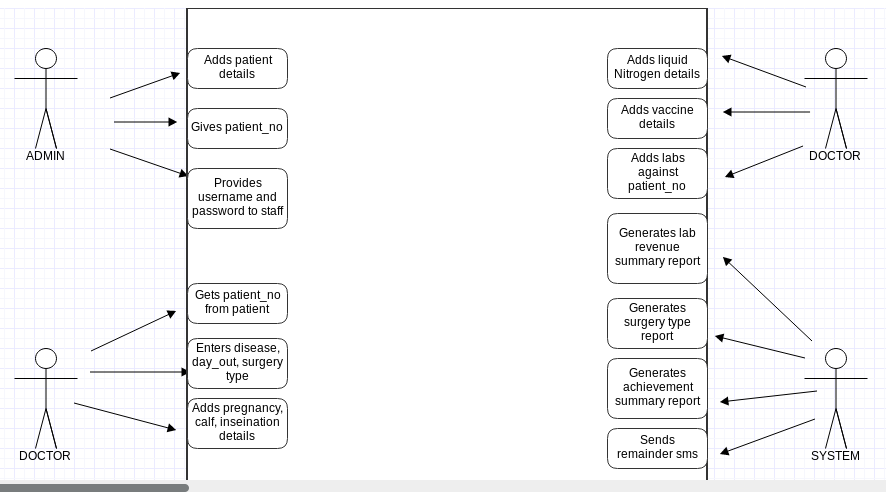
\includegraphics[width=\textwidth]{uml.png}}
	  \caption{Use case diagram}
	  \label{fig:usecase}
	\end{figure}
\end{center}  

\section{Data Model and Description}  
\subsection{Data Description}  
Data Requirements:The veterinary polyclinic data that is to be operated upon which includes all the patient details and details under different departments of the clinic.
The developed application should allow the doctor to login to the application using his sign in details and let him insert the details of a new patient.Any new details should be updated directly to the database.Final reports should be generated as per the doctor’s requirements showing all the statistical data for brief analysis.

\subsection{Data objects and Relationships}
Data objects and their major attributes and relationships among data objects are described using an ERD- like form.
 
 
\section{Functional Model and Description}  
The summary report, lab revenue reports and the surgery report will be generated from the following tables:
1. Patient table
2. Labs table

\subsection{Data Flow Diagram}  
\subsubsection{Level 0 Data Flow Diagram}
\begin{center}
	\begin{figure}[!htbp]
		\centering
		\fbox{\includegraphics[width=\textwidth]{dfd0.png}}
	  \caption{Data Flow diagram}
	  \label{fig:usecase}
	\end{figure}
\end{center}
\subsubsection{Level 1 Data Flow Diagram}
 



 
\subsection{Activity Diagram:}
 \begin{center}
	\begin{figure}[!htbp]
		\centering
		\fbox{\includegraphics[width=\textwidth]{activity.png}}
	  \caption{Activity diagram}
	  \label{fig:usecase}
	\end{figure}
\end{center}

\newpage
\subsection{Non Functional Requirements:}
\begin{itemize}
	\item	Interface Requirements
	\item	Performance Requirements
    \item	Software quality attributes such as availability [ related to Reliability], modifiability [includes portability, reusability, scalability] ,  		performance, security, testability and usability[includes self 			adaptability and user adaptability] 
\end{itemize} 

\subsection{State Diagram:}	
  State Transition Diagram\\
Fig.\ref{fig:state-dig} example shows the state transition diagram of Cloud SDK. The states are
represented in ovals and state of system gets changed when certain events occur. The transitions from one state to the other are represented by arrows. The Figure    shows important states and events that occur while creating new project.

\begin{center}
	\begin{figure}[!htbp]
		\centering
		\fbox{\includegraphics[width=\textwidth]{statechart.png}}
	  \caption{State transition diagram}
	  \label{fig:state-dig}
	\end{figure}
\end{center} 
 
 \subsection{Design Constraints}	
 \begin{itemize}
 \item The doctors should be educated on how to use the system,
\item Hardware requirements:
(i) Processor: Intel Core i3
(ii) OS Type: 64 bit
(iii) RAM: 4 GB
\item Software requirements:
 Netbeans IDE, Apache Tomcat, Mysql DBMS, Client side scripting: HTML, CSS
Server side scripting: PHP
 \end{itemize}


 \subsection{Software Interface Description}	
 \begin{enumerate}[1.]
\item Login Page:
\begin{enumerate}[(i)]
\item A login page for authorization.
\item Input details compared with the saved staff record.
\end{enumerate}

\item Registration Module:
\begin{enumerate}[(i)]
\item For registering new client details.
\item Client details saved in a database.
\end{enumerate}

\item Departments/inventory module:
\begin{enumerate}[(i)]
\item Mysql database for every department.
\item Records can be viewed, updated for all departments.
\item Inventory details are maintained in a separate database.
\end{enumerate}

\item Report generation/statistics:
\begin{enumerate}[(i)]
\item Final reports generated.
\end{enumerate}

\item Messaging System:
\begin{enumerate}[(i)]
\item Text messages sent to patients.
\item Textlocal.in used for subscription.
\end{enumerate}


\end{enumerate}  





\chapter{Detailed Design Document using Appendix A and B}
 \section{Introduction}  
In veterinary polyclinics, the hospital records are managed manually. The records are hand-
written and the reports are made by the doctors.We have proposed a system that will automate
these manual tasks. Since it is a web application, the doctors can access it remotely.The
application coordinates the activities of different branches of the hospital and communicates
between them.This will ease the processes of hospital management. Since the system is
providing statistics and reports of the hospital records, much of the work will be reduced.
 
\section{Architectural Design}  
	A description of the program architecture is presented. Subsystem design or Block diagram,Package Diagram,Deployment diagram with description is to be presented.

 
  \begin{center}
	\begin{figure}[!htbp]
		\centering
		\fbox{\includegraphics[width=470pt]{architecture.png}}
	  \caption{Architecture diagram}
	  \label{fig:arch-dig}
	\end{figure}
\end{center} 


\section{Data design (using Appendices A and B)}   
Quality Attributes:
\begin{enumerate}[(a)]
\item Design Qualities: Conceptual Intergrity,Maintainability,Reusability
\item Runtime Qualities: Availibility,Performance
\item System Qualities: Supportabilty,Testability
\end{enumerate}



\subsection{Global data structure}
Doctor’s page and admin page will be available at all times.
\subsection{Temporary data structure}
Interim php files are created for handling the connectivity and querying.
\subsection{Database description}
\begin{enumerate}[1.]
\item Patient table: Stores the details of patients like ownername, address, phoneno etc.
\item ai table: Stores the details of artificial insemination.
\item infertility table: Stores the infertility table details.
\item labs table: stores the details about the labs that are used by the patients.
\item calfdetails table: stores the details about the calf birth.
\item vaccination: keeps the records of vaccination.
\item pregnancy table: stores the information about the pregnancy details.
\item liquid nitrogen table: stores the stock information of the liquid nitrogen.
\item admin: stores the login details of the staff
\end{enumerate}




\section{Component Design} 
Class diagrams, Interaction Diagrams, Algorithms. Description of each component description required.
\subsection{Class Diagram}
 \begin{center}
	\begin{figure}[!htbp]
		\centering
		\fbox{\includegraphics[width=450pt]{class.png}}
		\fbox{\includegraphics[width=450pt]{class2.png}}
	  \caption{Class Diagram}
	  \label{fig:class-dig}
	\end{figure}
\end{center} 
 
\chapter{Project Implementation}
  \section{Introduction}
  We have implemented this project using various tools and technology like HTML, CSS for client side scripting, PHP for server side scripting, Apache 2 server that works on the central system and MySQL database.
  \section{Tools and Technologies Used}
  \begin{enumerate}[1.]
 \item HTML:
HTML stands for Hyper Text Markup Language, which is the most widely used language on Web to develop web pages. A web form or HTML form on a web page allows a user to enter data that is sent to a server for processing. Forms can resemble paper or database forms because web users fill out the forms using checkboxes, radio buttons, or text fields. Used for writing forms which form the basis of data storing from the user.
\item CSS:
A CSS framework is a pre-prepared software framework that is meant to allow for easier, more standards-compliant web design using the Cascading Style Sheets language. Most of these frameworks contain at least a grid. More functional frameworks also come with more features and additional JavaScript based functions, but are mostly design oriented and unobtrusive. This differentiates these from functional and full JavaScript frameworks. Used for styling of the User Interface.
\item PHP: 
Hypertext Preprocessor (or simply PHP) is a server-side scripting language designed for web development but also used as a general-purpose programming language. PHP code may be embedded into HTML code, or it can be used in combination with various web template systems, web content management systems, and web frameworks. PHP code is usually processed by a PHP interpreter implemented as a module in the web server or as a Common Gateway Interface (CGI) executable. The web server combines the results of the interpreted and executed PHP code, which may be any type of data, including images, with the generated web page. Used for back end for connectivity and transactions.
\item MySQL:
MySQL is an open-source relational database management system (RDBMS). MySQL is a central component of the LAMP open-source web application software stack (and other "AMP" stacks). LAMP is an acronym for "Linux, Apache, MySQL, Perl/PHP/Python". MySQL is also used in many high-profile, large-scale websites, including Google (though not for searches), Facebook, Twitter, Flickr, and YouTube. Used for storing the main data for the system.
  \end{enumerate}
  

  \section{Methodologies/Algorithm Details}
  \subsection{Algorithm 1/Pseudo Code}
  \begin{enumerate}[1.]
\item	Start 
\item	Enter the URL
\item	Login as admin
\item	Case \\
4.1	Enter new patient \\
4.2	Enter details \\
4.3	Submit \\
4.4	Update database 
\item	View details \\
5.1	View all the patients
\item	Enter new doctor \\
6.1	Add new doctor details \\
6.2	Create new entry
\item	Logout
  \end{enumerate}



  \subsection{Algorithm 2/Pseudo Code}
  \begin{enumerate}
  \item Start
\item	Enter the URL
\item	Login as doctor
\item	Case \\
4.1.	Select from different departments \\
4.2.	Enter patient details \\
4.3.	Submit
\item	Calculate fees
\item	View reports
\item	Logout
  \end{enumerate}

  \section{Verification and Validation for Acceptance}
  This system has been built based on the requirement of the Polyclinic on the lines of their current system which is inefficient. Our system caters to the needs of the polyclinic thereby providing additional functions which thoroughly improves the quality and quantity of the deliverables.
  
  
\chapter{Software Testing}
 \section{Type of Testing Used}
   There are different types of testing we use in our project. Some testing types are as follows:
   \begin{enumerate}[1.]
  \item	UNIT TESTING: 
Unit testing is the testing in which we do an individual unit or group of related units. It falls under the class of white box testing. It is often done by the programmer to test that the unit she has implemented is producing expected output against given input. So here we do the individual function testing.

\item	INTEGRATION TESTING: 
Integration testing is testing in which a group of components are combined to produce output. Also, the interaction between software and hardware is tested in integration testing if software and hardware components have any relation. It may fall under both white box testing and black box testing.

\item	FUNCTIONAL TESTING: 
Functional testing is the testing to ensure that the specified functionality required in the system requirements works. It falls under the class of black box testing.

\item	SYSTEM SYSTEMS: 
System testing is the testing to ensure that by putting the software in different environments (e.g., Operating Systems) it still works. System testing is done with full system implementation and environment. It falls under the class of black box testing.

\item	PERFORMANCE TESTING: 
Performance testing is the testing to assess the speed and effectiveness of the system and to make sure it is generating results within a specified time as in performance requirements. It falls under the class of black box testing. It checks the performance of our system.

\item	USABILITY TESTING: 
Usability testing is performed to the perspective of the client, to evaluate how the GUI is user-friendly? How easily can the client learn? After learning how to use, how proficiently can the client perform? How pleasing is it to use its design? This falls under the class of black box testing.

\item	ACCEPTANCE TESTING: 
Acceptance testing is often done by the customer to ensure that the delivered product meets the requirements and works as the customer expected. It falls under the class of black box testing.
   \end{enumerate}


   \section{Test Cases and Test Results}
  \begin{table}[!htbp]
\begin{center}
%\def\arraystretch{1.5}
\def\arraystretch{1.5}
\begin{tabularx}{\textwidth}{| X | X | X | X | X |}
\hline
\multirow{1}{*}{Test case No.} & \multirow{1}{*}{Description}	& \multirow{1}{*}{Precondition} & \multirow{1}{*}{Expected result } & \multirow{1}{*}{actual result}  \\ \hline
TC1	& To check whether user has logged in	& User should be on login page	& Login Successful &	Login Successful \\ \hline
TC2	& Check username and password are valid or not &	User should be on login page &	Display Error message (Wrong username or password) &	Display Error message (Wrong username or password) \\ \hline
TC3 &	Check all the fields are filled or not	& All the fields should be properly filled &	Entered data is correct	& Entered data is correct \\ \hline
TC4	& To check if the count is given against the correct type of animal &	Provide separate input methods for each animal type &	Data provided successfully	& Data provided successfully \\ \hline
TC5	& Check whether patients data is successfully stored in the database or not &	Data should be stored in the database	& Data stored successfully &	Data stored successfully \\ \hline
TC6	& Performance testing for page loading time	& Page shall be loaded within acceptable time ran &	Page loaded in minimum response time &	Page loaded in minimum response time \\ \hline
TC7 &	Performance testing for database query execution time &	Database query execution time shall be within acceptable time range &	File retrieval is fast &	File retrieval is fast \\  \hline

\end{tabularx}
\end{center}
\caption{Test Cases}
\label{tab:usecase}
\end{table}
   
\chapter{Results}
\section{Screen shots}
\subsection{Login Page}
 \begin{center}
	\begin{figure}[!htbp]
		\centering
		\fbox{\includegraphics[width=500pt]{login.png}}
	  \caption{Login Page}
	  \label{fig:Login page}
	\end{figure}
\end{center} 
\newpage
\subsection{Admin Login}
 \begin{center}
	\begin{figure}[!htbp]
		\centering
		\fbox{\includegraphics[width=480pt]{admin1.png}}
		\fbox{\includegraphics[width=480pt]{admin.png}}
		
	  \caption{Admin Login}
	  \label{fig:Admin Login}
	\end{figure}
\end{center}

\newpage
\subsection{Doctor Login}
 \begin{center}
	\begin{figure}[!htbp]
		\centering
		\fbox{\includegraphics[width=480pt]{doc1.png}}
		\fbox{\includegraphics[width=480pt]{doc2.png}}
		
	  \caption{Doctor Login}
	  \label{fig:Doctor Login}
	\end{figure}
\end{center}

\newpage
\section{Outputs}
\subsection{Reports}
 \begin{center}
	\begin{figure}[!htbp]
		\centering
		\fbox{\includegraphics[width=480pt]{doc3.png}}
		\fbox{\includegraphics[width=480pt]{doc4.png}}
		
		
	  \caption{Reports}
	  \label{fig:Reports}
	\end{figure}
\end{center}
\fbox{\includegraphics[width=480pt]{doc5.png}}
		\fbox{\includegraphics[width=480pt]{doc6.png}}
\newpage
\subsection{Messaging}
 \begin{center}
	\begin{figure}[!htbp]
		\centering
		\fbox{\includegraphics[width=300pt]{mobile.png}}
		
		
		
	  \caption{Messaging}
	  \label{fig:Messaging}
	\end{figure}
\end{center}
    
\chapter{Deployment and Maintenance}
     \section{Installation and un-installation}
     \begin{enumerate}
     \item The server machine need Apache HTTPD Server installed.
     \item The server should have MYsql database system installed.
     \item Subscription to Textlocal.in.
     \item Subscription to URL domain(optional)
     
     
     
     \end{enumerate}
     
    
     
 \chapter{Conclusion and future scope}
\begin{enumerate}
\item CONCLUSION :\\ \\
Thus,the digital system gets implemented and the traditional hand written system gets atomised.Separate user interfaces for doctors and administrator is created to simplify the work.The project also considers the Inventory management aspect of the veterinary polyclinic.A systematic approach is followed for the process starting from insemination stage ,infertility,pregnancy diagnosis and finally the calf birth.The reports get generated as per the users requirements which reduce a lot of work for the doctors.An automated messaging system is implemented which helps in notifying the patients about their next infertility check up which is due in 3 months.Hence,this way our project becomes the first web application for a veterinary polyclinic in Maharashtra.Hence,this is our small contribution to the Digital India campaign.\\ \\
\item FUTURE SCOPE :
\begin{enumerate}[1.]
\item A mobile application can be developed for the same.
\item Medical Inventory can be added as a part of clinical dbms.
\item The patients can make appointments using the system will be a part of future development.
\end{enumerate}



\end{enumerate}
 
% \bibliographystyle{plain}

\bibliographystyle{ieeetr}
\bibliography{biblo}

\begin{appendices}

\chapter{References}

\begin{enumerate}[{[1]}]
\item K. S. Sim, T. K. Kho, F. S. Abas, F. F. Ting, V. Teh and C. S. Ee, “Computerized Brain Database Management System for Radiological Department in Hospital,” International Conference of Robotics, Automation and Sciences(ICORAS), 2016.
\item Paulo Silva, Cesar Quintas, J´ulio Duarte, Manuel Santos, Jos´e Neves, Ant´onio Abelha and Jos´e Machado, “Hospital database workload and fault forecasting,” IEEE-EMBS Conference on Biomedical Engineering and Sciences, pp. 63-68, 2012.
\item Jeong-cheol Jeon, Jaehwa Chung, “Developing a Prototype of REST-based Database Application for Shipbuilding Industry: A Case Study,” International Conference on Platform Technology and Service (PlatCon), pp. 1-6, 2017.
\item Cheng Zhi, “The Web database application system optimization research,” Seventh International Conference onMeasuring Technology and Mechatronics Automation, pp. 1329-1332, 2015.
\end{enumerate}


% \chapter{ALGORITHMIC DESIGN}
\chapter{Laboratory assignments on Project Analysis of Algorithmic Design}
\begin{itemize}
\item To develop the problem under consideration and justify feasibilty using
concepts of knowledge canvas and IDEA Matrix.\\


\begin{table}[!htbp]
\begin{center}
  
  \begin{tabular}{|p{3cm}| p{3cm}|p{3cm}|p{3cm}|}
\hline
 I & D & E & A \\ 
\hline

Increase : Efficiency & Drive :Disadvantages in handwritten records & Educate :Educate the doctors on how to use the system. & Accelerate : Report generation process\\
 
\hline
Improve :Storage,
Time efficiency,
Fetch time,
 & Deliver :Automated reports,
Web application.
 & Evaluate :Testing for errors& Artists :Doctors,Admin \\
 \hline
Ignore :Internet unavailability & Decrease :Search time.& Eliminate :Redundancy & Avoid :Arithmetic errors\\
\hline
\end{tabular}
 \caption { IDEA Matrix }
 \label{tab:imatrix}
\end{center}
\end{table}

\item Project problem statement feasibility assessment using NP-Hard, NP-Complete or satisfy ability issues using modern algebra and/or relevant mathematical models. \\ 



Application for managing veterinary polyclinic

\begin{enumerate}
\item Aim: Project problem statement feasibility assessment using NP-Hard, NP-Complete or satisfiability issues using modern algebra.
\item NP class : A problem is assigned to the NP (nondeterministic polynomial time) class if it is solvable in polynomial time by a nondeterministic Turing machine. A P-problem (whose solution time is bounded by a polynomial) is always also NP.
\item NP-Complete Class: In computational complexity theory, an NP-complete decision problem is one which is in the NP complexity class and which is also NP-hard. In this context, NP stands for "nondeterministic polynomial time". The set of NP-complete problems is often denoted by NP-C or NPC.
\item NP Hard Class: The complexity class of decision problems that are intrinsically harder than those that can be solved by a nondeterministic Turing machine in polynomial time. P Class: It contains all decision problems that can be solved by a deterministic Turing machine using a polynomial amount of computation time, or polynomial time.
\item Complexity of query processing

In practice, we deal with the data complexity of the Query Evaluation Problem for Relational Calculus,
because we typically have a small fixed collection of queries to answer (while the database instances vary).
The complexity of query evaluation problem depends uopn two factors- the query complexity and the data complexity. The combined complexity is given as NP-complete.
\item Client-server application

the proposed system is a 3-tier application.
It involves client server communication. The communication problems are reduced to NP-complete problems using Graph theory.

Thus the overall system complexity becomes NP complete.
\end{enumerate}















\end{itemize}



\chapter{Project Planner}
\label{app:plan}
\subsection{Project Plan}
 \begin{center}
	\begin{figure}[!htbp]
		\centering
		\fbox{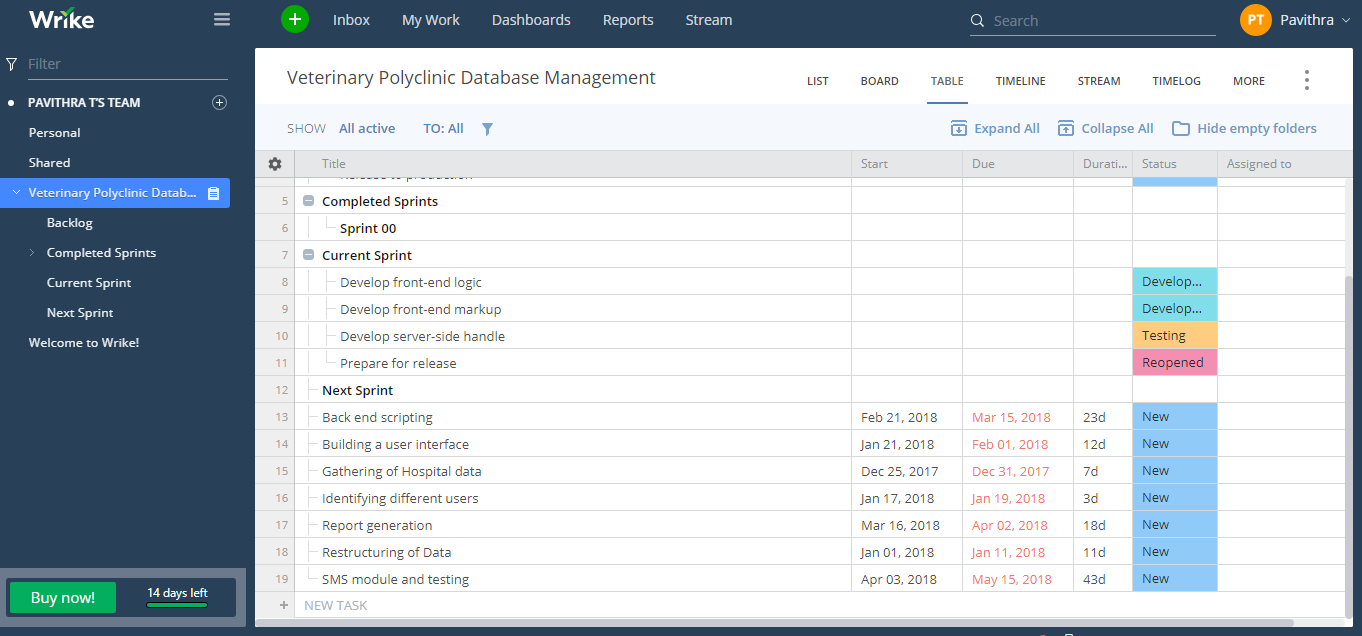
\includegraphics[width=500pt]{plan1.png}}
		\fbox{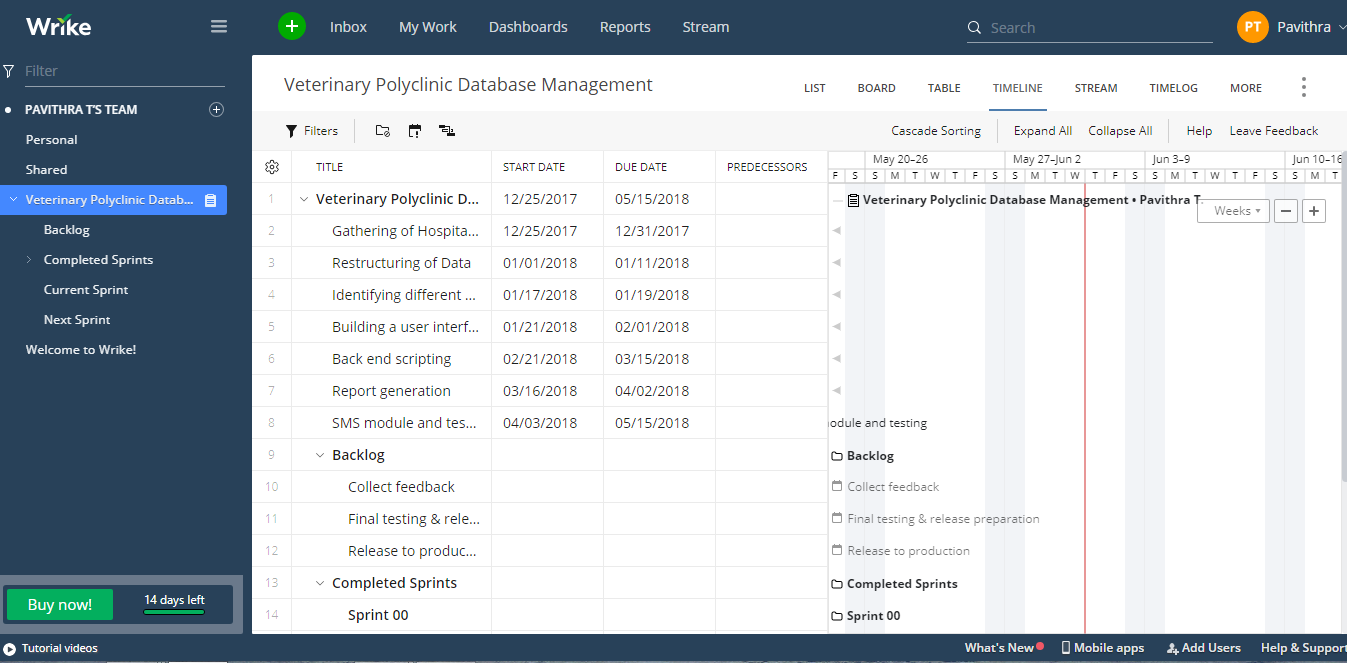
\includegraphics[width=500pt]{plan2.png}}
		
		 \caption{Project Plan}
	  \label{fig:Project Plan}
	\end{figure}
\end{center}

\newpage

\subsection{Project Plan}
 \begin{center}
	\begin{figure}[!htbp]
		\centering
		
		\fbox{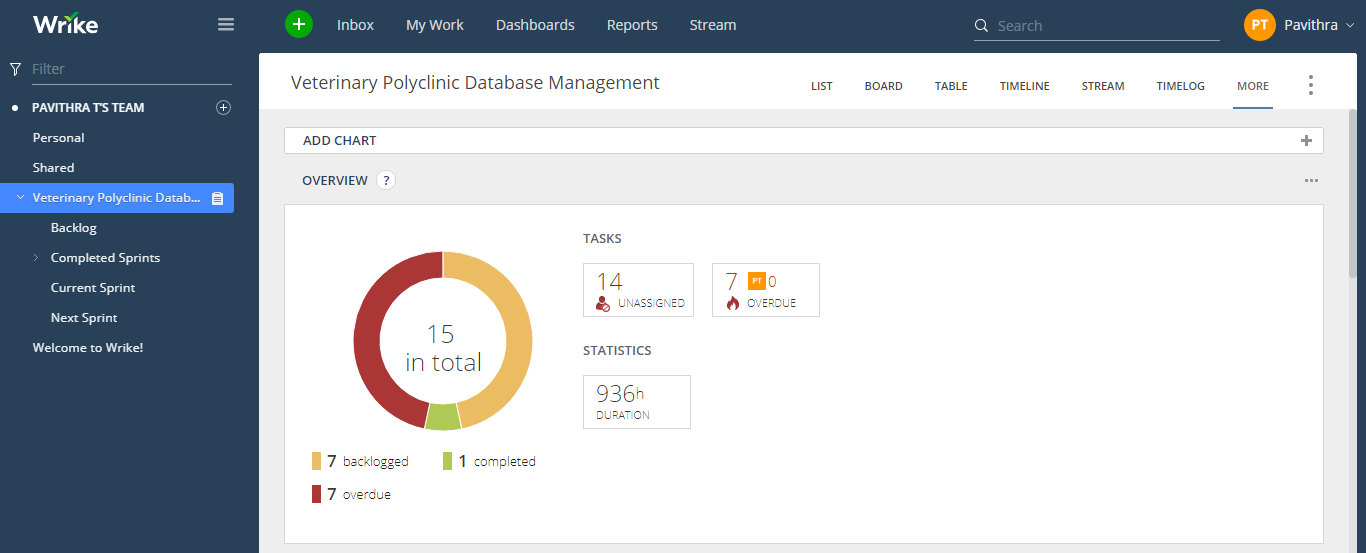
\includegraphics[width=500pt]{plan3.png}}
		\fbox{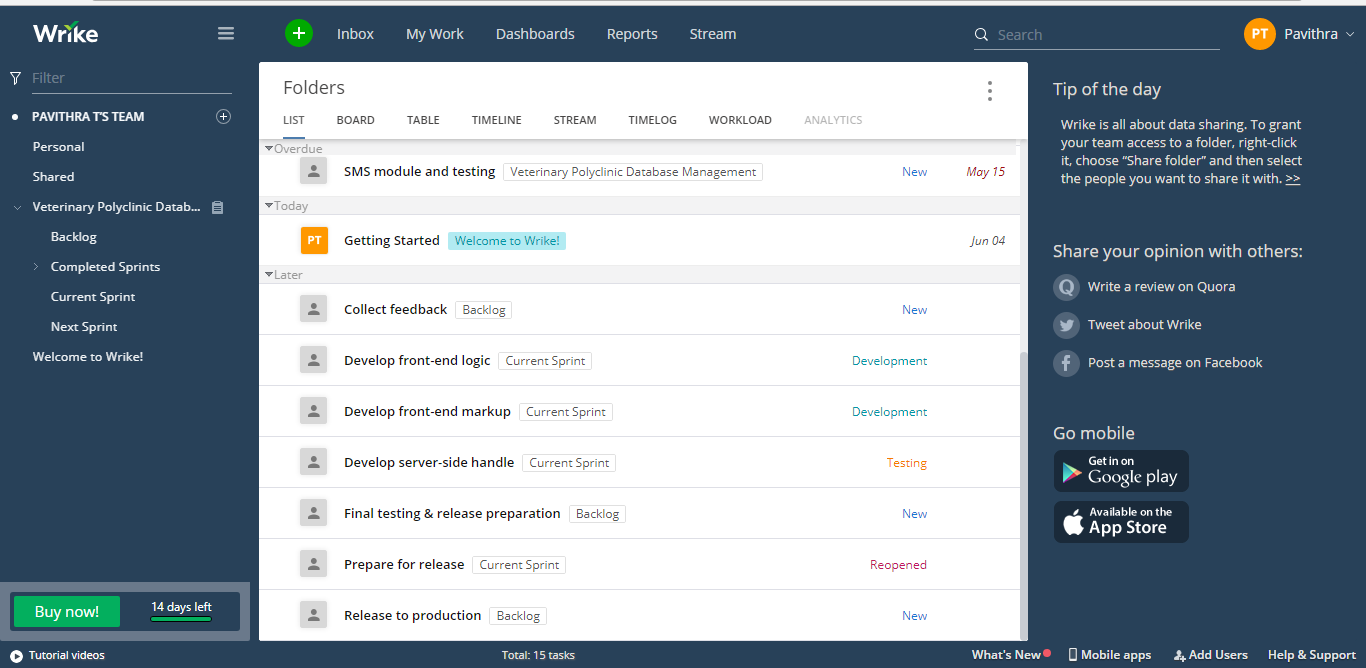
\includegraphics[width=500pt]{plan4.png}}
		 \caption{Project Plan}
	  \label{fig:Project Plan}
	\end{figure}
\end{center}









\chapter{Plagiarism Report}
Plagiarism report
\subsection{Plagiarism Report}
 \begin{center}
	\begin{figure}[!htbp]
		\centering
		\fbox{\includegraphics[width=400pt]{plag.png}}
		
		
		
	  \caption{Plagiarism Report}
	  \label{fig:Plagiarism Report}
	\end{figure}
\end{center}
\chapter{ Term-II Project Laboratory Assignments}
\begin{enumerate}
\item Review of design and necessary corrective actions taking into consideration the feedback report of Term I assessment, and other competitions/conferences participated like IIT, Central Universities, University Conferences or equivalent centers of excellence etc.

\begin{enumerate}[(i.)]
\item	Registration module: 
The ‘Admin’ will log-in to the system and enter the details of the patient. On clicking the submit button, the details get stored into the ‘patient’ database. 
Staff (doctors) details are added by the ‘Admin’. Unique usernames and passwords can be set by the Staff. 
\item	SDLC Model followed:
The software development life cycle model followed is the ‘Waterfall Model’. The Waterfall model involves the following phases – Gathering requirements, designing, implementation, verification, testing and maintenance.
\item	Deployment:
Local machines belonging to the same network are connected to the server. Server’s ip address is used to connect locally. 
\item	Completeness:
The project is NP Complete. 
\item Testing: 
Use of Selenium testing tool to test the test cases of log-in, report generation and submitting the forms. 
\item	Multiusers:
Use of sessions to provide multi-user environment. Different views provided to different users based on their ‘Status’.

\end{enumerate}

\item Project workstation selection, installations along with setup and installation report preparations.

\begin{enumerate}[(i.)]
\item	Project workstation selection:\\
System specifications of developmental machine: \\
Processor – Intel® Core™ i3-5010U CPU @ 2.10GHz  2.10 GHz,
Installed memory (RAM) – 8.00 GB,
System type – 64-bit Operating System, x84-based processor,
Operating System details – Linux Fedora 20 

\item	Software requirements: (client)\\
Any machine with any modern operating system that supports modern web browsers. Latest operating system versions, web browsers versions are preferred for efficient working.
\item	Hardware requirements: (min)\\
Processor - Intel Pentium 2009,
Speed – 2GHz,
No. of cores – 2
\item	Software requirements: (server)\\
i.	MySql database system should be installed.\\
ii.	Apache Httpd server should be installed.\\
iii.	Internet connectivity should be set up.\\

\item	Setup:\\
i.	Set up a wireless network connection.\\
ii.	Connect the local clients to the same network.\\
iii.	Type the IP address of the server and the login page at the web browser of the client.\\
iv.	The connection to the server is established when the login page is viewed at the client’s side.\\
v.	The system can now be used by logging in.


\end{enumerate}
\item Programming of the project functions, interfaces and GUI (if any) as per 1 st Term term-work submission using corrective actions recommended in Term-I assessment of Term-work.\\
\begin{enumerate}
\item The system is a web-application. Its first module is the access verification module.
The details of the system users along with their login credentials are stored in a database at the server side. The users can access the system only after authentication.
The system has two types of dedicated users:
•	Admin
•	Doctors

The system functions are user-specific.
\item Functions for admin
\begin{enumerate}[1.]
\item Add patient
When a new patient arrives, enter the basic details of the owner and patient. These details get stored in a database and can be accessed by the doctors on demand.
\item 	Add new doctor
When there is a need of adding a new doctor or removing an old one, the admin can enter username and create a new entry or delete one from the database.
\item Update lab test rates and vaccination rates
The polyclinic has different labs. The patients are charged as per the treatment in these labs.
	Also, the polyclinic maintains and makes provision for certain vaccinations.
	Using this functionality it can set/update rates for these vaccinations/labs.


\end{enumerate}
\newpage
\subsection{Code Snippet}
 \begin{center}
	\begin{figure}[!htbp]
		\centering
		\fbox{\includegraphics[width=500pt]{1.png}}
		
		
		
	  \caption{Code Snippet}
	  \label{fig:Code Snippet}
	\end{figure}
\end{center}
\item Functions for doctor
\begin{enumerate}[1.]
\item Adding patient details
When a patient arrives at the doctor, the doctor accesses his basic details from the database.
He diagnoses the animal and treats him or provides treatment details. Doctor’s module is not a heavy one since he has to focus more on treatment of the patient.
This includes mentioning of disease and suggesting the type of surgery if needed.
This is implemented using checkboxes and textboxes.
\item Listing the patients
If the doctors want to see the patients recorded for the day the can switch to this tab.
\item Listing animals for vaccination
Entering the number of different types of animals that have arrived at the hospital for the purpose of vaccination. These numbers are stored against different animals in the database.
These are then used to calculate the cost of vaccination for an owner.
\item 	Insemination
Entering the cattle details for Artificial Insemination.
Here, an automated messaging module is implemented which notifies the owner of  the pregnancy checkup visit date after the gestation period.
\item 	Pregnancy
The doctor has to enter the details of pregnancy checkup of the cattle.
\item 	Infertility
Details of inferitlity of the cattle are entered here.
\item  Calf Birth
Details of the calf being born are entered. This helps in estimating the cattle population.
\item 	Maintaining of nitrogen supply
The details of the nitrogen dealer and the stock details are entered here.
\item 	Labs
The labs which will be assigned for the treatment of any animal are specified here with the help of checkboxes.
This is required to calculate the fees for treatment
\item 	Reporting
Different types of reports are generated. This is time based reporting. The doctor enters the period for which he wants the reports and the result will be displayed.








\end{enumerate}
\newpage
\subsection{Code Snippet}
 \begin{center}
	\begin{figure}[!htbp]
		\centering
		\fbox{\includegraphics[width=500pt]{3.png}}
		
		
		
	  \caption{Code Snippet}
	  \label{fig:Code Snippet}
	\end{figure}
\end{center}

\item 	Automated messaging module
\newpage
\subsection{Code Snippet}
 \begin{center}
	\begin{figure}[!htbp]
		\centering
		\fbox{\includegraphics[width=500pt]{4.png}}
		
		
		
	  \caption{Code Snippet}
	  \label{fig:Code Snippet}
	\end{figure}
\end{center}





\end{enumerate}





\end{enumerate}
\chapter{Information of Project Group Members}

\begin{enumerate}
\item Name : SHALINI PRASANNA \hspace{50 mm}\includegraphics[width=90pt]{shalini.jpg}
\item Date of Birth : 03/08/1996
\item Gender : Female
\item Permanent Address : Kumar presidency phase 2,1101,Meera Nagar,koregaon park.
\item E-Mail : shalini.prasanna@cumminscollege.in
\item Mobile/Contact No. : 9923124646
\item Placement Details : Not Placed


\end{enumerate}
\newpage
\begin{enumerate}
\item Name : T. PAVITHRA \hspace{50 mm}\includegraphics[width=90pt]{pavi.jpg}
\item Date of Birth : 10/04/1996
\item Gender : Female
\item Permanent Address :Bloom 203, My World, Opp to Cummins Office, Balewadi High Street, Baner Road, Pune 
\item E-Mail : t.pavithra@cumminscollege.in
\item Mobile/Contact No. : 9960822880
\item Placement Details : Cybage


\end{enumerate}
\newpage
\begin{enumerate}
\item Name : SUPRIYA WAGHMARE \hspace{50 mm}\includegraphics[width=90pt]{sup.jpg}
\item Date of Birth : 26/01/1996
\item Gender : Female
\item Permanent Address : B-51,Ramnagar Colony,Ghugus,Chandrapur.
\item E-Mail : supriya.waghmare@cumminscollege.in
\item Mobile/Contact No. : 7028291278
\item Placement Details : Infosys

\newpage
\end{enumerate}
\begin{enumerate}
\item Name : ASHLESHA WAIKOS \hspace{50 mm}\includegraphics[width=90pt]{ash.jpg}
\item Date of Birth : 30/04/1996
\item Gender : Female
\item Permanent Address : G801, Jacobina, Nyati Equatorial, Bavdhan, Pune.
\item E-Mail : ashlesha.waikos@cumminscollege.in
\item Mobile/Contact No. : 9764486484
\item Placement Details : Not Placed


\end{enumerate}
\end{appendices}

\end{document}
